\documentclass{article}

\usepackage[utf8]{inputenc}
\usepackage[T1]{fontenc}
\usepackage[spanish]{babel}
\usepackage{times}
\usepackage{wrapfig}
\usepackage{lmodern}
\usepackage{mathtools}
\usepackage{graphicx}
\usepackage[utf8]{inputenc}
\usepackage{color}
\usepackage{hyperref}
\usepackage{fancyhdr,lipsum}


\hypersetup{
    colorlinks=true, %set true if you want colored links
    linktoc=all,     %set to all if you want both sections and subsections linked
    linkcolor=blue,  %choose some color if you want links to stand out
}
\urlstyle{same}

\title{Presupuesto}
\author{Antonio Muñoz Cubero}
\date{3 de Noviembre de 2020} 

\begin{document}
  \maketitle
  \pagenumbering{gobble}
  \pagestyle{fancy}
  
  \newpage
    \tableofcontents
    \lhead[Presupuesto SSII]{Presupuesto SSII}
    \lfoot[IES Francisco De Los Rios]{IES Francisco De Los Rios}
  
  \newpage
    \pagenumbering{roman}

  \newpage
    \section{Enunciado}
      Utilizando como base el trabajo realizado en el ejercicio anterior, realizar un diseño de equipo de escritorio empleando componentes reales que se encuentren en el mercado. Se puede emplear como lista de materiales 
      y precios cualquier tienda real física o de Internet (PC Componentes, PC Box, etc.). Justificar en todo momento la compatibilidad de los componentes empleados con la placa base escogida.
      \begin{itemize}
        \item Realizar un dimensionamiento correcto de la potencia necesaria para la fuente de alimentación.
        \item Realizar el calculo del coste de material empleando una hoja de calculo (excel o similar).
      \end{itemize}
      Se debe entregar el documento en formato PDF, Entregar también el presupuesto elaborado con la hoja de calculo (puede estar también impreso en formato PDF).
      \\\\
      \subsection{Aclaraciones}
      Este trabajo es una continuación del anterior, que en mi caso fue la \href{https://github.com/ErTonix12/DAM/blob/main/1%C2%BA/SI/Placa_Base_Documentaci%C3%B3n/build/Placa_Base_Documentacion.pdf}{documentación de la 
      placa base}, que puede ver pulsando en el enlace. (No puede ser visualizado online en el navegador \textit{Microsoft EDGE}.)
      \\
      En este presupuesto utilizaré la placa base anterior, y construiré un \textit{PC} en base a ella, siendo este presupuesto válido en caso de hacerlo efectivo, pues las compatibilidad de todos los componentes están más
       que testados.
  \newpage
    \section{Procesador}
      \subsection{Descripción}
        Para el apartado del \textit{procesador} he elegido uno de los procesadores más potentes del mercado y uno de los más potentes dentro del fabricante \textit{AMD}, se trada de \textbf{AMD Ryzen 9 3900X}.
        \\
        \begin{minipage}{0.5\textwidth}
          Este procesador pertenece a la tercena generación de procesadores AMD Ryzen, este procesdor dispone de \textbf{12 nucles y 24 hilos}, con una frecuencia base del procesador de \textbf{3.8 GHz} y una velocidad 
          máxima de \textbf{4.6 GHz}. El procesador está desbloqueado para realizar overclock, pero en caso de que queramos hacerlo, deberíamos cambiar el disipador de fábrica, en mi caso, en este presupuesto cambiaremos 
          de disipador, que lo veremos más adelante.
        \end{minipage}
        \begin{minipage}{\textwidth}
          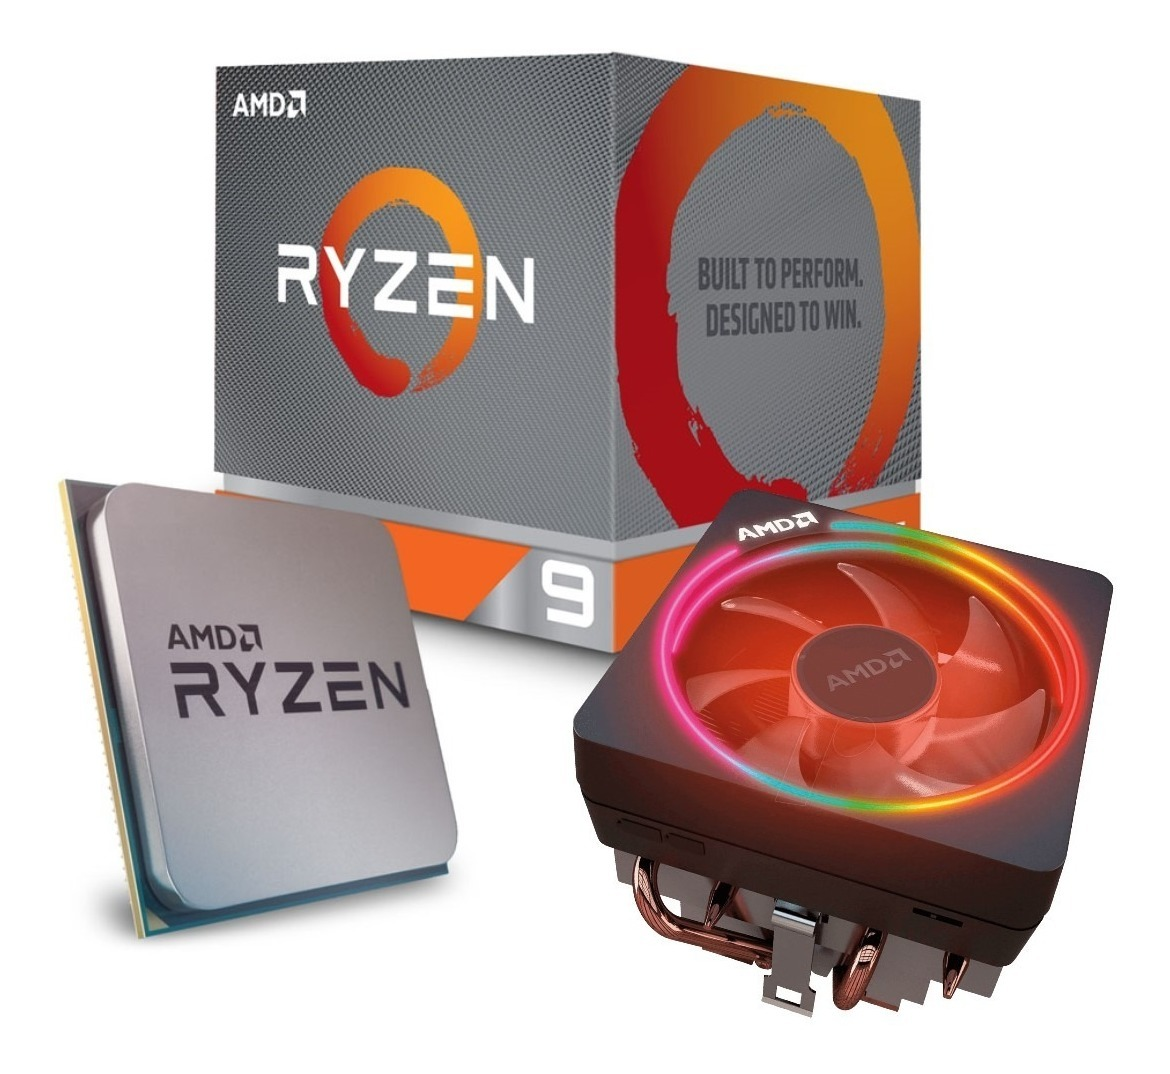
\includegraphics[scale=0.2]{img/procesador.jpg}
        \end{minipage}
      \subsection{Precio}
        En lo que respecta al precio, podemos observar un descenso paulatino en el mismo, quedándose ahora mismo en \textbf{455,90€} en la página \href{https://www.pccomponentes.com/amd-ryzen-9-3900x-38-ghz-box}{Pccomponentes}, 
        que puede ver, pulsando en el enlace.
        \\
        \begin{figure}[h]
          \centering
          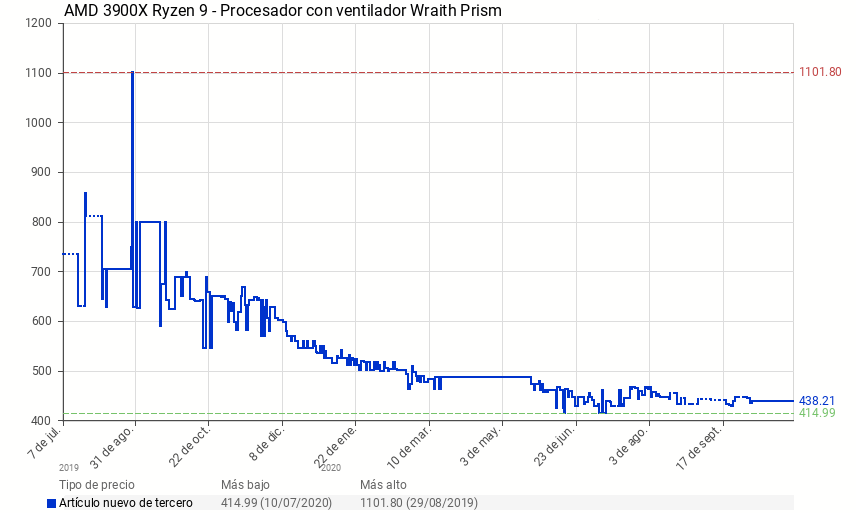
\includegraphics[scale = 0.4]{img/grafica_procesador.png}
        \end{figure}
  
  \newpage
    \section{Placa Base}
      \subsection{Descripción}
        Para este apartado, usaremos la placa base \textbf{B550 Aorus Master} del fabricante \textit{Gigabyte}, esta la usé para hacer la documentación de la práctica anterior, que puede verse pulsando \href{https://github.com/ErTonix12/DAM/blob/main/1%C2%BA/SI/Placa_Base_Documentaci%C3%B3n/build/Placa_Base_Documentacion.pdf}{aquí}.
        \\
        \begin{minipage}{0.5\textwidth}
          Esta placa tiene un socket \textbf{AM4} que soporta la \textit{3º Gen de AMD Ryzen} por lo tanto, es completamente compatible con el procesador elegido. La chipset \textbf{B550} es uno de los más potentes en el socket AM4, por lo tanto, tenemos suficiente base para 
          poder montar un équipo tope de gama. La placa incluye \textbf{PCIe 4.0, Tarjeta de Sonido, Tarjeta de Red y Tarjeta gráfica}, pero no tendremos que preocuparnos de la tarjeta gráfica, ya que más adelante incluiremos una 
          en nuestro presupuesto.
        \end{minipage}
        \begin{minipage}{\textwidth}
          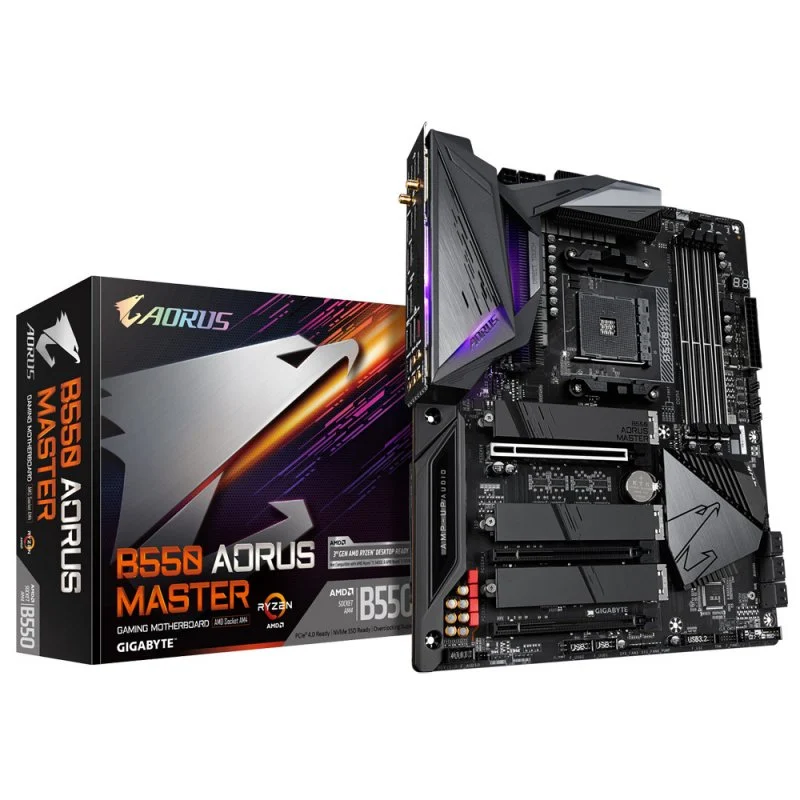
\includegraphics[scale=0.4]{img/placa_base.png}
        \end{minipage}
      \subsection{Precio}
        En cuanto al precio, esta placa base al ser un producto cuyo lanzamiento se realizó hace unos meses, no podemos ver una evolución óptima de su gráfica de valor, pero podemos decir que la podemos encontrar por \textbf{294,90€} en la página 
        \href{https://www.pccomponentes.com/gigabyte-b550-aorus-master}{Pccomponentes} y puede consultar más información pulsando en el enlace.
        \\
        \begin{figure}[h]
          \centering
          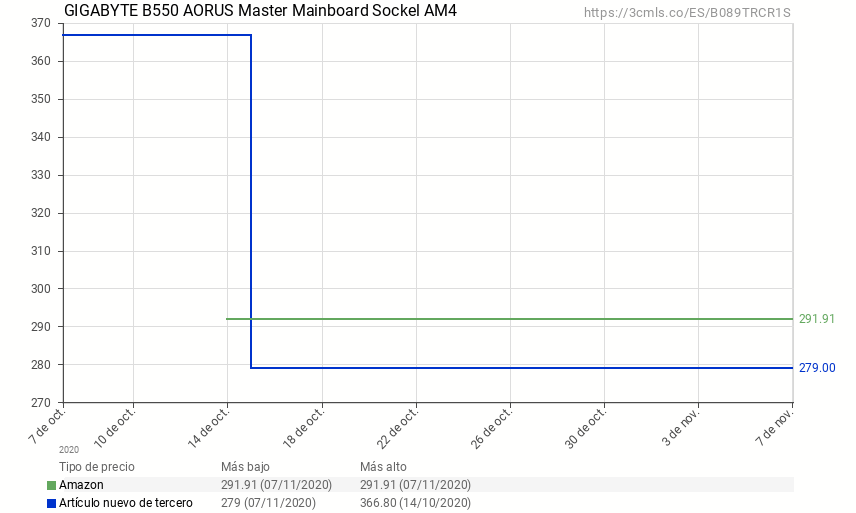
\includegraphics[scale = 0.3]{img/grafica_placa.png}
        \end{figure}

  \newpage
    \section{Memoria RAM}
      \subsection{Descripción}
        Para la Memoria RAM he optado por las \textbf{Corsair Dominator Platinum}, contando con dos módulos de 16GB haciendo un total de \textbf{32 GB de Memoria RAM}.
        \\
        \begin{minipage}{0.5\textwidth}
        Contamos con 2 módulos, por lo tanto, podemos beneficiarnos de la tecnología del \textbf{DUAL CHANNEL}, además son \textbf{DDR4} con velocidades de \textit{3200 MHz} por lo que nuestro ordenador no tendrá problema para compilar, ejecutar ni mover 
        cualquier programa que le echemos encima.
        \end{minipage}
        \begin{minipage}{\textwidth}
          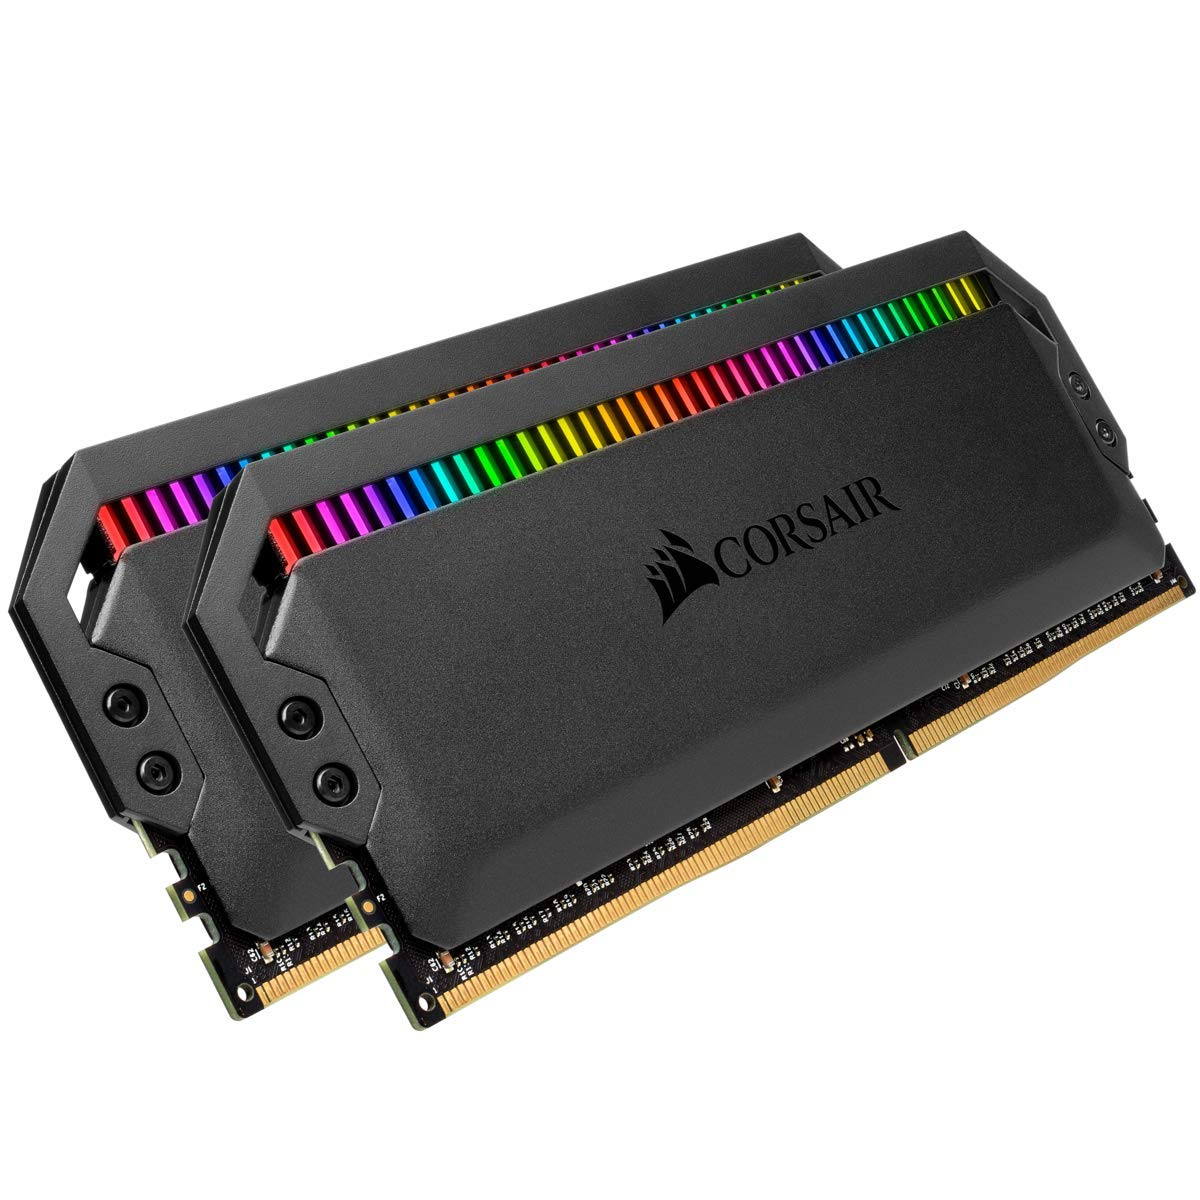
\includegraphics[scale = 0.2]{img/ram.png}
        \end{minipage}
      \subsection{Precio}
        El precio de la memoriam RAM ha oscilado en gran medida durante el paso del tiempo como poedemos observar en el gráfico, hoy en día este pack lo podemos encontrar por \textbf{208,99€} en 
        \href{https://www.pccomponentes.com/corsair-dominator-platinum-rgb-ddr4-3200-pc4-25600-32gb-2x16gb-cl16}{Pccomponentes} y puede consultar más información pulsando en el enlace.
        \\
        \begin{figure}[h]
          \centering
          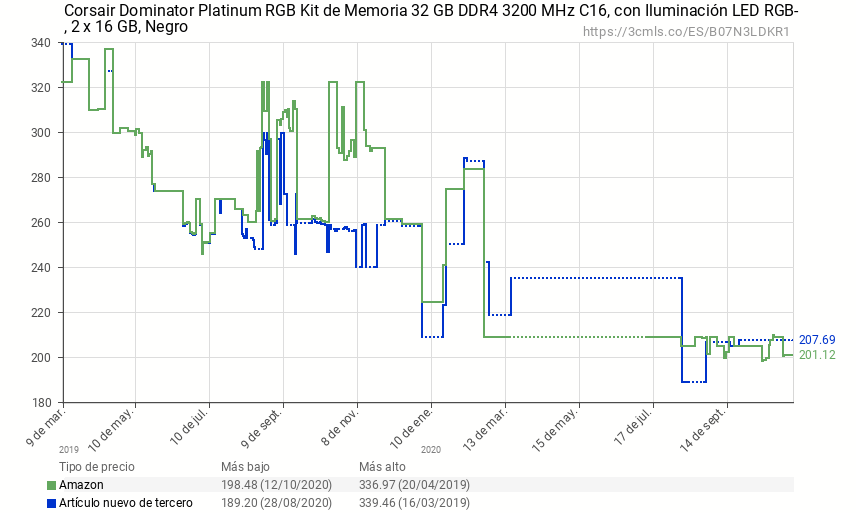
\includegraphics[scale = 0.3]{img/grafica_ram.png}
        \end{figure}

  \newpage
    \section{Disipador de la CPU}
      \subsection{Descripción}
        Como bien hablamos en el apartado de la CPU, no nos queríamos conformar con el disipador de stock, así que hemos puesto una refrigeración líquida para mantener a raya la temperatura de nuestro procesador. Se trata de 
        \textbf{Corsair Hydro H100x}.
        
        \begin{minipage}{0.5\textwidth}
          Este pack de refrigeración líquida de Corsarir es compatible con el zócalo AM4 por lo tanto no tendremos problemas de instalación,  trae su propio radiador con dos ventiladores que funcionan a altas revoluciones, manteniendo
            una silenciosa eficiencia.
        \end{minipage}
        \begin{minipage}{\textwidth}
          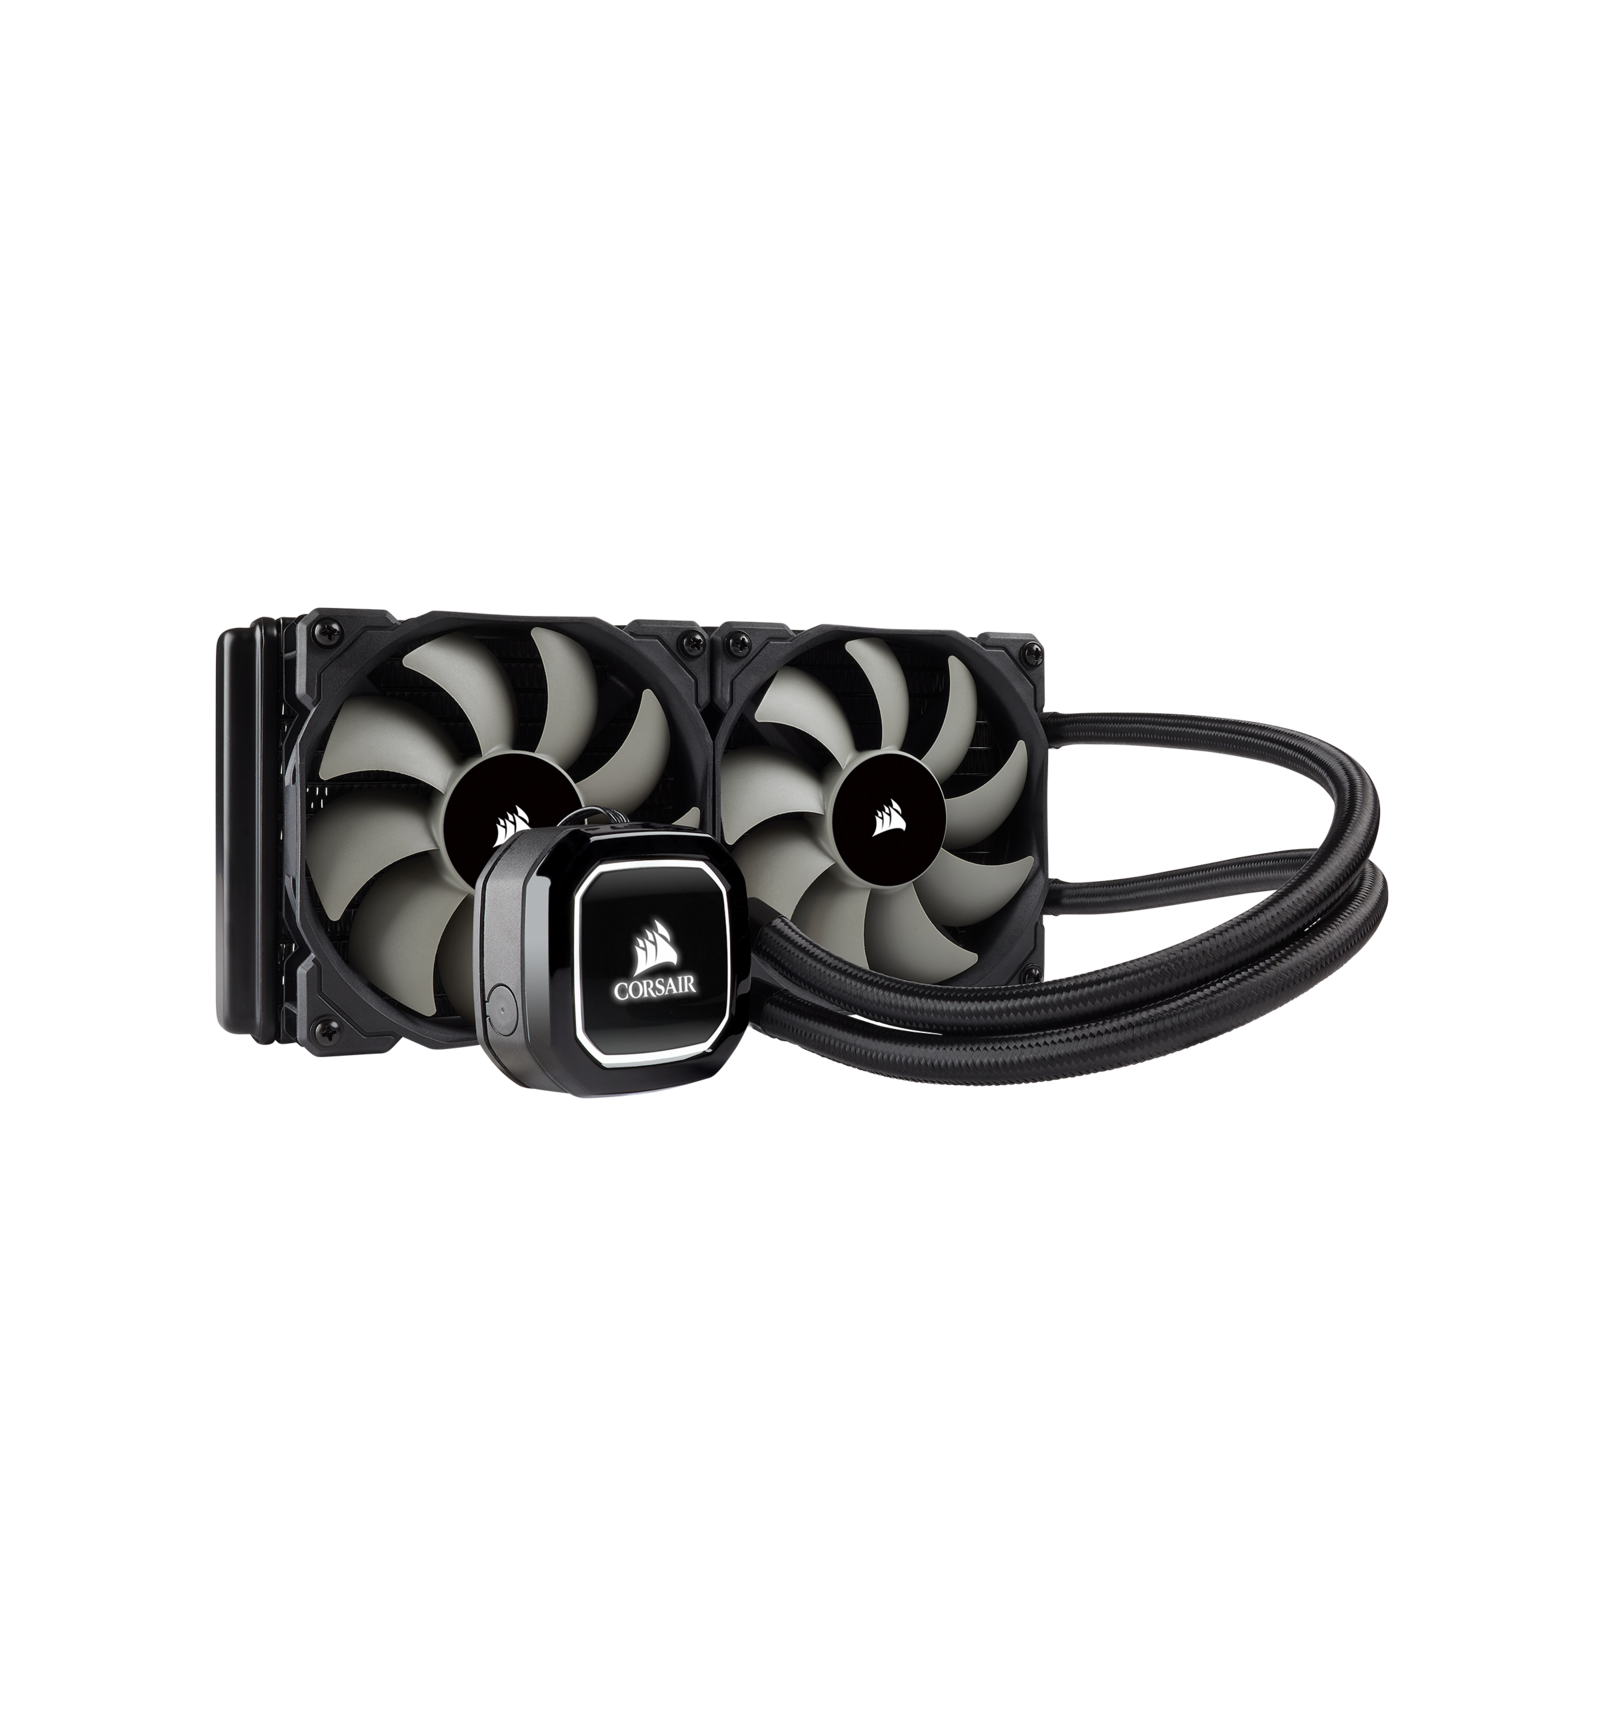
\includegraphics[scale=0.15]{img/refrigeracion.png}
        \end{minipage}
      \subsection{Precio}
        El precio de este kit de refrigeración es de \textbf{94 ,90€} y puede consultarse en 
        \href{https://www.pccomponentes.com/corsair-hydro-h100x-kit-de-refrigeracion-liquida}{Pccomponentes} y puede consultar más información pulsando en el enlace.
        
  \newpage
    \section{Disco Duro}
      \subsection{Descripción}
        Para el almacenamiento he optado por el \textbf{Samsung 970 EVO Plus} de \textit{500GB SSD NVMe M.2}.
        \\\\
        \begin{minipage}{0.5\textwidth}
          Considero que es suficiente almacenamiento para tener el S.O o incluso varios, con sus programas, moltimedia y demás, hoy en día todos podemos tener a mano discos duro externos para almacenar el contenido multimedia, y así no hacemos sufrir tanto al disco. Al ser un \textbf{SSD} no da una velocidad de lectura de \textbf{3500 MB/s} suficiente para arrancat Windows en menos de 10s.
        \end{minipage}
        \begin{minipage}{\textwidth}
          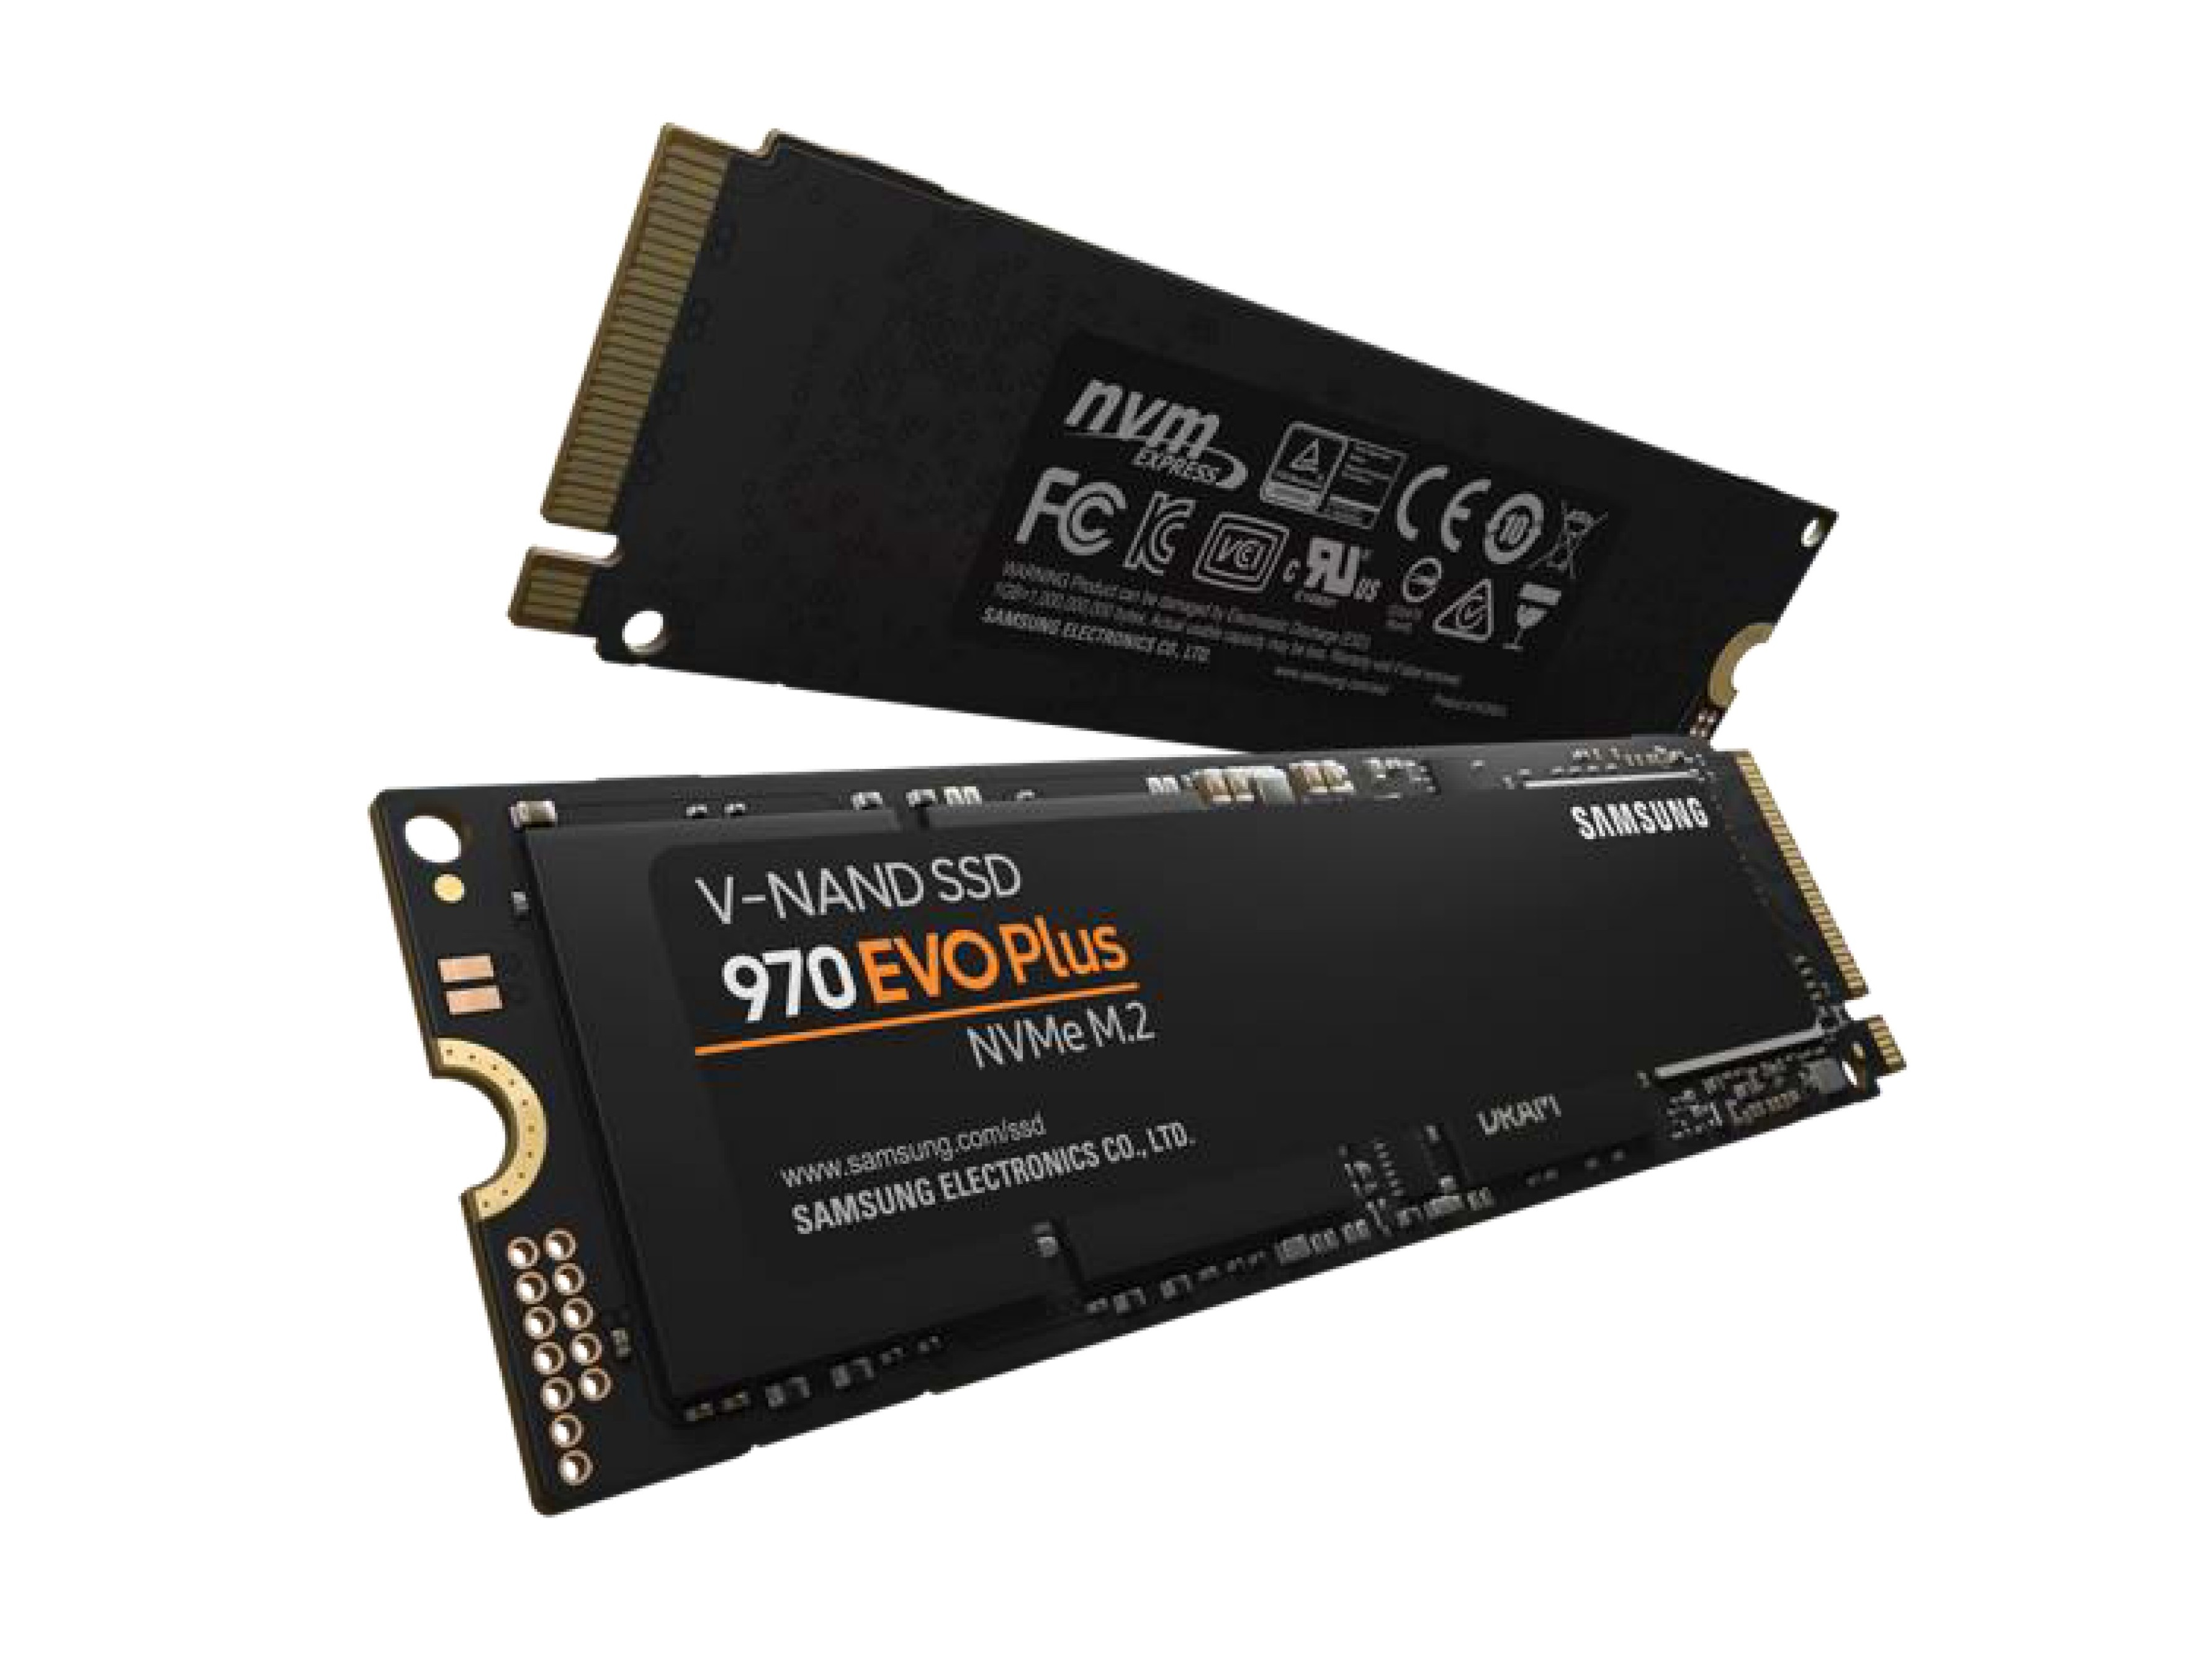
\includegraphics[scale=0.5]{img/disco_duro.jpg}
        \end{minipage}
      \subsection{Precio}
        El precio del disco ha variado mucho en los último meses, ahora lo podemos encontrar a 
        \textbf{109 ,99€} y puede consultarse en 
        \href{https://www.pccomponentes.com/samsung-970-evo-plus-500gb-ssd-nvme-m2}{Pccomponentes} y puede consultar más información pulsando en el enlace.
        \\
        \begin{figure}[h]
          \centering
          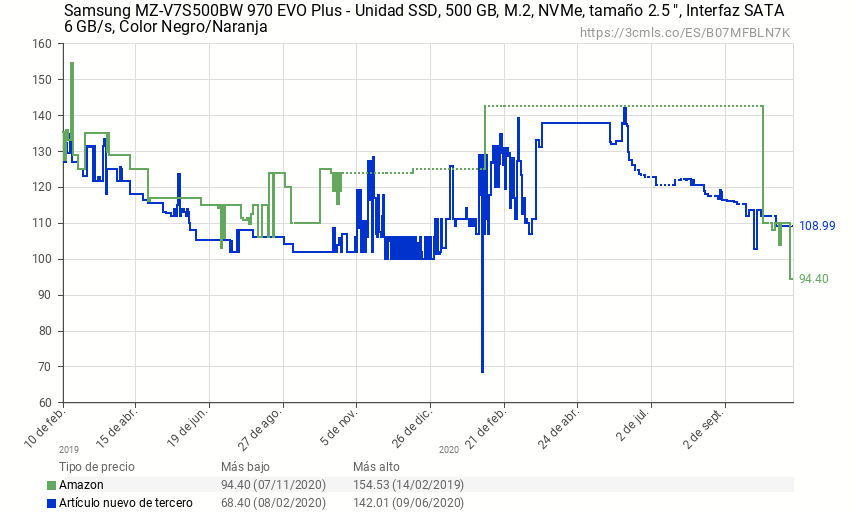
\includegraphics[scale = 0.4]{img/grafica_disco.png}
        \end{figure}

  \newpage
    \section{Tarjeta Gráfica}
      \subsection{Descripción}
        Para el procesamiento gráfico he elegido la GPU de la marca \textit{Gigabyte} en concreto el modelo \textbf{AMD Radeon RX 5700 XT}.
        \\
        \begin{minipage}{0.5\textwidth}
         Este modelo cuenta con una capacidad de \textit{8GB de VRAM GDDR6}, soporta \textbf{PCIe 4.0} así aprovechamos esa ventaja que nos brindaba la placa base, también nos puede alcanzar a dar una resolución de hasta 8K.
        \end{minipage}
        \begin{minipage}{\textwidth}
          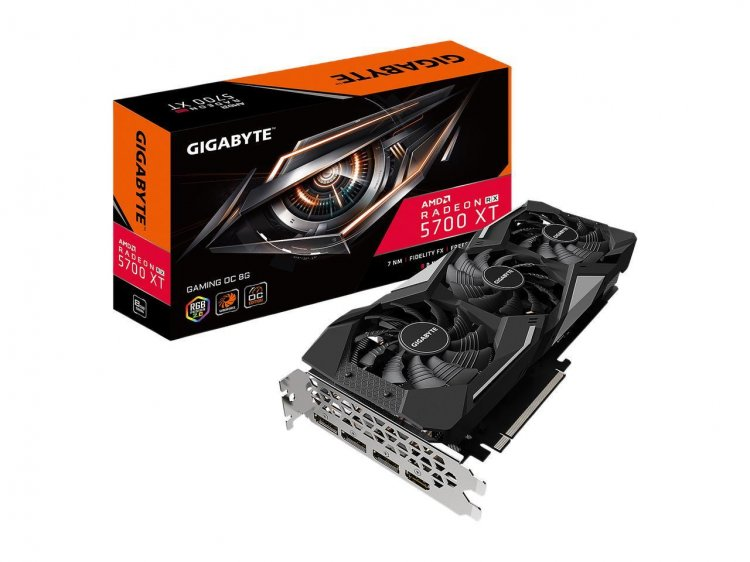
\includegraphics[scale=0.35]{img/grafica.jpg}
        \end{minipage}
      \subsection{Precio}
        El precio de la tarjeta varía bastante, oscilando entre los 400€ y los 500€, ahora mismo podemos encontrarla a un precio de 
        \textbf{429,90€} y puede consultarse en 
        \href{https://www.pccomponentes.com/gigabyte-amd-radeon-rx-5700-xt-gaming-oc-8gb-gddr6}{Pccomponentes} y puede consultar más información pulsando en el enlace.
        \\
        \begin{figure}[h]
          \centering
          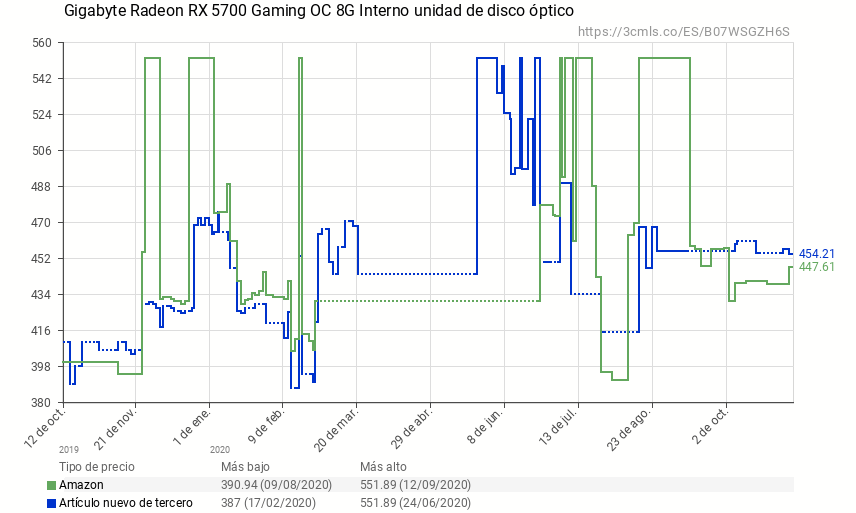
\includegraphics[scale = 0.4]{img/grafica_grafica.png}
        \end{figure}
          


          

\end{document}

